\documentclass[a4paper]{book}
\usepackage{fullpage}

\usepackage[utf8]{inputenc}
\usepackage[T1]{fontenc}
\usepackage[francais]{babel}

\usepackage{latexsym}
\usepackage{fancyhdr}
\usepackage{makeidx}
\usepackage{graphics}
\usepackage{graphicx}
\usepackage{float} %
\usepackage{caption} %
\usepackage{longtable}
\usepackage{moreverb}
\usepackage{listings}

\newcommand{\altarica}{{\sc AltaRica}}

\begin{document}

\title{Master 1, Conceptions Formelles\\
Projet du module \altarica\\
Synthèse (assistée) d'un contrôleur du niveau d'une cuve}

\date{}

\author{Craeye Nathalie \and Faltrept Bérénice \and Lejeune David}

\maketitle

\chapter{Le sujet}
\section{Cahier des charges}

Le système que l'on souhaite concevoir est composé~:
\begin{itemize}
\item d'un réservoir contenant {\bf toujours} suffisamment d'eau pour alimenter l'exploitation,
\item d'une cuve,
\item de deux canalisations parfaites amont reliant le réservoir à la cuve, et permettant d'amener l'eau à la cuve,
\item d'une canalisation parfaite aval permettant de vider l'eau de la cuve,
\item chaque canalisation est équipée d'une vanne commandable, afin de réguler l'alimentation et la vidange de la cuve,
\item d'un contrôleur.
\end{itemize}

\subsection{Détails techniques}

\subsubsection{La vanne}
Les vannes sont toutes de même type, elles possèdent trois niveaux de débits correspondant à trois diamètres d'ouverture~: 0 correspond à la vanne fermée, 1 au diamètre intermédiaire et 2 à la vanne complètement ouverte. Les vannes sont commandables par les deux instructions {\tt inc} et {\tt dec} qui respectivement augmente et diminue l'ouverture. Malheureusement, la vanne est sujet à défaillance sur sollicitation, auquel cas le système de commande devient inopérant, la vanne est désormais pour toujours avec la même ouverture.

\subsubsection{La Cuve}
Elle est munie de $nbSensors$ capteurs (au moins quatre) situés à $nbSensors$ hauteurs qui permettent de délimiter $nbSensors+1$ zones. La zone 0 est comprise entre le niveau 0 et le niveau du capteur le plus bas; la zone 1 est comprise entre ce premier capteur et le second, et ainsi de suite.

Elle possède en amont un orifice pour la remplir limité à un débit de 4, et en aval un orifice pour la vider limité à un débit de 2.  

\subsubsection{Le contrôleur}
Il commande les vannes avec les objectifs suivants ordonnés par importance~:
\begin{enumerate}
\item Le système ne doit pas se bloquer, et le niveau de la cuve ne doit jamais atteindre les zones 0 ou $nbSensors$.
\item Le débit de la vanne aval doit être le plus important possible.
\end{enumerate}

On fera également l'hypothèse que les commandes ne prennent pas de temps, et qu'entre deux pannes et/ou cycle {\em temporel}, le contrôleur à toujours le temps de donner au moins un ordre. Réciproquement, on fera l'hypothèse que le système à toujours le temps de réagir entre deux commandes.

\subsubsection{Les débits}
Les règles suivantes résument l'évolution du niveau de l'eau dans la cuve~:
\begin{itemize}
\item Si $(amont > aval)$ alors au temps suivant, le niveau aura augmenté d'une unité.
\item Si $(amont < aval)$ alors au temps suivant, le niveau aura baissé d'une unité.
\item Si $(amont = aval = 0)$ alors au temps suivant, le niveau n'aura pas changé.
\item Si $(amont = aval > 0)$ alors au temps suivant, le niveau pourra~:
  \begin{itemize}
  \item avoir augmenté d'une unité,
  \item avoir baissé d'une unité,
  \item être resté le même.
  \end{itemize}
\end{itemize}

\section{L'étude}

\subsection{Rappel méthodologique}
Comme indiqué en cours, le calcul par point fixe du contrôleur est exact, mais l'opération de projection effectuée ensuite peut perdre de l'information et générer un contrôleur qui n'est pas satisfaisant. Plus précisemment, le contrôleur \altarica\ généré~:
\begin{itemize}
\item ne garanti pas la non accessibilité des \emph{Situations Redoutées}.
\item ne garanti pas l'absence de \emph{nouvelles situations de blocages}.
\end{itemize}

Dans le cas ou il existe toujours \emph{des situations de blocages ou redoutées}, vous pouvez au choix~:
\begin{enumerate}
\item Corriger manuellement le contrôleur calculé (sans doute très difficile).
\item Itérer le processus du calcul du contrôleur jusqu'à stabilisation du résultat obtenu. 
  \begin{itemize}
  \item Si le contrôleur obtenu est sans blocage et sans situation redoutée, il est alors correct.
  \item Si le contrôleur obtenu contient toujours des blocages ou des situations redoutées, c'est que le contrôleur initial n'est pas assez performant, mais rien de garanti que l'on soit capable de fournir ce premier contrôleur suffisemment performant.
  \end{itemize}
\end{enumerate}

{\bf Remarque} : Pour vos calculs, vous pouvez utiliser au choix les commandes~:
\begin{itemize}
\item {\tt altarica-studio xxx.alt xxx.spe}
\item {\tt arc -b xxx.alt xxx.spe}
\item {\tt make} pour utiliser le fichier GNUmakefile fourni.
\end{itemize}

\subsection{Le travail a réaliser}

Avant de calculer les contrôleurs, vous devez répondre aux questions suivantes.
\begin{enumerate}
\item Expliquez le rôle de la constante $nbFailures$ et de la contrainte, présente dans le composant {\tt System}, $nbFailures >= (V[0].fail + V[1].fail + V[2].fail)$.
\item Expliquez le rôle du composant {\tt ValveVirtual} et de son utilisation dans le composant {\tt CtrlVV}, afin de remplacer le composant {\tt Ctrl} utilisé en travaux dirigés.
\end{enumerate}

L'étude consiste à étudier le système suivant deux paramètres~:
\begin{enumerate}
\item $nbFailures$~: une constante qui est une borne pour le nombre de vannes pouvant tomber en panne.
\item Le contrôleur initial qui peut être soit {\tt Ctrl}, soit {\tt CtrlVV}.
\end{enumerate}

Pour chacun des huit systèmes étudiés, vous devez décrire votre méthodologie pour calculer les différents contrôleurs et répondre aux questions suivantes~:

\begin{enumerate}
\item Est-il possible de contrôler en évitant les blocages et les situations critiques ?
\item Si oui, donnez quelques caractéristiques de ce contrôleur, si non, expliquez pourquoi.
\item Est-il possible de contrôler en optimisant le débit aval et en évitant les blocages et les situations critiques ?
\item Si oui, donnez quelques caractéristiques de ce contrôleur, si non, expliquez pourquoi.
\end{enumerate}


\chapter{Le rapport}

Pour les deux questions qui suivent, nous avons analysé essentiellement les fichiers GNUmakefile à la racine du projet, system.alt, parameters.alt, tank.alt, test.alt, et CtrlVV.alt.
En effet nous avons remarqués dans le fichier GNUmakefile, qu'à l'utilisation de la commande "make" on génère toutes les configurations possibles du système sur lequel nous travaillons : 
une première boucle assure la génération des fichiers pour tous les contrôleurs ( Ctrl et CtrlVV). Pour chacun d'entre eux, une boucle va produire des fichiers associés aux nombres de pannes.

\section{Rôle de la constante {\tt nbFailures} (2 points)}

$nbFailures$ est la constante qui récupère le nombre de pannes prédéfini au lancement d'une configuration du système. En effet, elle est initialisée en prenant la valeur de la variable $nbPannes$ dans le système en cours. \\
La contrainte, et assertion, du composant {\tt System} $nbFailures >= (V[0].fail + V[1].fail + V[2].fail)$ permet d'assurer que le modèle lancé par l'utilisateur a une configuration cohérente, c'est-à-dire que le nombre de valves en panne dans le modèle en cours sera compris entre 0 (meilleur cas : il n'y aurait aucune valve en panne) et 3 (pire cas : les trois valves, i.e toutes, existantes du système sont en panne). \\

\section{Rôle des composants {\tt ValveVirtual} et {\tt CtrlVV} (4 points)}

$ValveVirtual$ est le composant permettant de simuler une valve parfaite, autrement dit sans panne. En l'intégrant au modèle, via CtrlVV, on peut alors confirmer la cohérence du modèle indépendemment de la gestion des pannes. \\
Pour chaque niveau d'itération, on va donc créer une version virtuelle, sans panne, pour contrôler le système mais aussi créer la version avec Ctrl et Valve qui assure la gestion des pannes.

\section{Résultats avec le contrôleur initial {\tt Ctrl}}

\subsection{Calcul d'un contrôleur}

\subsubsection{Avec 0 défaillance (1 point)}
\lstinputlisting{Res/System0FCtrl.res}
\lstinputlisting{Res/System0FCtrl0F1I.res}
\lstinputlisting{Res/System0FCtrl0F2I.res}
\lstinputlisting{Res/System0FCtrl0F3I.res}
\lstinputlisting{Res/System0FCtrl0F4I.res}
\paragraph{Interprétation des résultats}

On observe que sur les différentes itérations : excepté la première, elles sont toutes identiques. De plus, notre système n'a aucun deadlock et les situations redoutées n'existent plus après cette première tentative. Donc les modifications appliquées à partir de l'itération 1 sont concluantes et permettent d'obtenir un système que l'on peut supposer fiable.

\begin{itemize}
	\item Oui. À partir de l'itération 1, il n'y a plus de situation critique et nous n'avions aucun état puit. Or, dans cette situation, CtrlCanControl parvient à contrôler 27 transitions.
	\item Avec un débit aval de 0, on obtient moins de sommets. On présume donc qu'il est optimal d'avoir un débit de 0 puisque cela nous permet de n'avoir aucune situation critique en gérant moins de cas.

\end{itemize}

\subsubsection{Avec 1 défaillance (1 point)}
\lstinputlisting{Res/System1FCtrl.res}
\lstinputlisting{Res/System1FCtrl1F1I.res}
\lstinputlisting{Res/System1FCtrl1F2I.res}
\lstinputlisting{Res/System1FCtrl1F3I.res}
\lstinputlisting{Res/System1FCtrl1F4I.res}
\paragraph{Interprétation des résultats}

Nous voyons que comparé à la version 0 défaillance, l'itération initiale a beaucoup plus de situations redoutées possibles, ce qui est normal pour une situation avec une valve défaillante. \\
À la première itération, nous remarquons des états puits produits, et que les sommets pour lesquels le niveau d'eau est critique sont tous des deadlocks puisque SR est équivalent à deadlock. \\ 
Or, en utilisant Altarica studio on s'aperçoit que la trace des deadlock ne nous mènent qu'à 4 sommets. En affichant le graphe avec la commande $dot(any\_s, tr\_deadlock)$, on découvre que ces 4 cas sont lorsque le niveau de l'eau dans la cuve est débordant.

\begin{figure}[H]
  \centering
  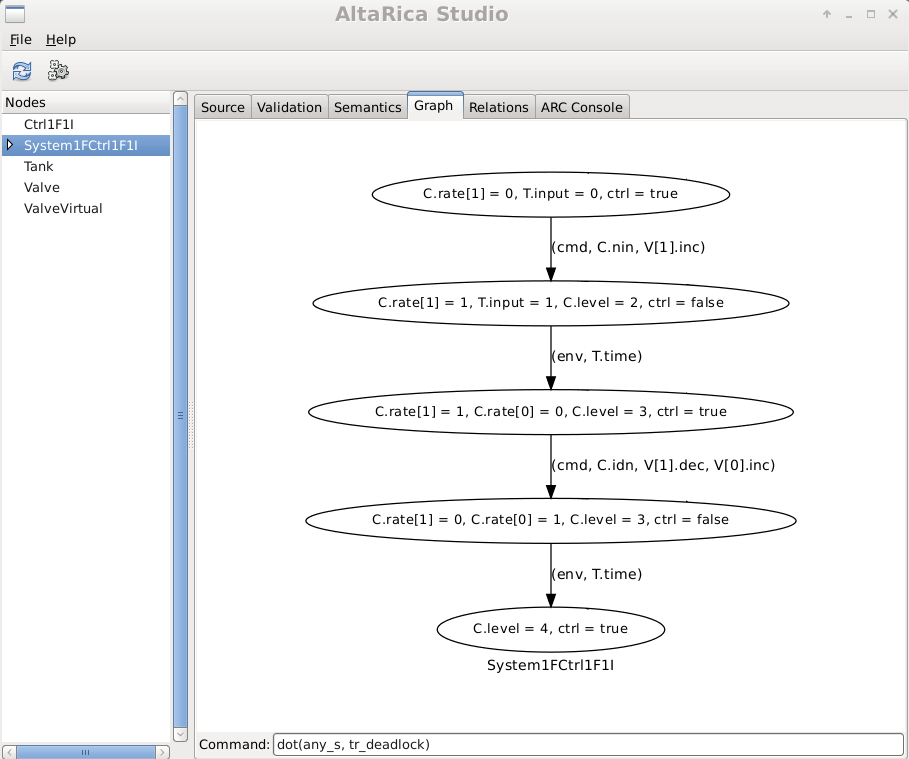
\includegraphics[width=14cm]{img/CtrlF1I1.png}
  %\caption{}
\end{figure}


La situation se stabilise à l'itération 2 : Par la suite, il n'y a plus de changement de valeurs. Mais avant ca, entre l'itération 1 et l'itération 2, on remarque le seul le nombre de transitions change, les états sont déjà stables.

\begin{itemize}
	\item En ayant une valve défaillante, on peut contrôler toutes les situations excepté les débordements de cuves, qui peuvent arriver quelle que soit la valve abîmée. Dans ce cas, on doit trouver une solution spécifique à ce problème : par exemple, garder une ouverture en haut de la cuve qui entrainerait une déperdition de l'eau le temps que l'on répare la valve.
	\item 

\end{itemize}
\subsubsection{Avec 2 défaillances (1 point)}
\lstinputlisting{Res/System2FCtrl.res}
\lstinputlisting{Res/System2FCtrl2F1I.res}
\lstinputlisting{Res/System2FCtrl2F2I.res}
\lstinputlisting{Res/System2FCtrl2F3I.res}
\lstinputlisting{Res/System2FCtrl2F4I.res}
\paragraph{Interprétation des résultats}

\subsubsection{Avec 3 défaillances (1 point)}
\lstinputlisting{Res/System3FCtrl.res}
\lstinputlisting{Res/System3FCtrl3F1I.res}
\lstinputlisting{Res/System3FCtrl3F2I.res}
\lstinputlisting{Res/System3FCtrl3F3I.res}
\lstinputlisting{Res/System3FCtrl3F4I.res}
\paragraph{Interprétation des résultats}

\subsection{Calcul des contrôleurs optimisés (2 points)}

\section{Résultats avec le contrôleur initial {\tt CtrlVV}}

\subsection{Calcul d'un contrôleur}

\subsubsection{Avec 0 défaillance (1 point)}
\lstinputlisting{Res/System0FCtrlVV.res}
\lstinputlisting{Res/System0FCtrlVV0F1I.res}
\lstinputlisting{Res/System0FCtrlVV0F2I.res}
\lstinputlisting{Res/System0FCtrlVV0F3I.res}
\lstinputlisting{Res/System0FCtrlVV0F4I.res}
\paragraph{Interprétation des résultats}

\subsubsection{Avec 1 défaillance (1 point)}
\lstinputlisting{Res/System1FCtrlVV.res}
\lstinputlisting{Res/System1FCtrlVV1F1I.res}
\lstinputlisting{Res/System1FCtrlVV1F2I.res}
\lstinputlisting{Res/System1FCtrlVV1F3I.res}
\lstinputlisting{Res/System1FCtrlVV1F4I.res}
\paragraph{Interprétation des résultats}

\subsubsection{Avec 2 défaillances (1 point)}
\lstinputlisting{Res/System2FCtrlVV.res}
\lstinputlisting{Res/System2FCtrlVV2F1I.res}
\lstinputlisting{Res/System2FCtrlVV2F2I.res}
\lstinputlisting{Res/System2FCtrlVV2F3I.res}
\lstinputlisting{Res/System2FCtrlVV2F4I.res}
\paragraph{Interprétation des résultats}

\subsubsection{Avec 3 défaillances (1 point)}
\lstinputlisting{Res/System3FCtrlVV.res}
\lstinputlisting{Res/System3FCtrlVV3F1I.res}
\lstinputlisting{Res/System3FCtrlVV3F2I.res}
\lstinputlisting{Res/System3FCtrlVV3F3I.res}
\lstinputlisting{Res/System3FCtrlVV3F4I.res}
\paragraph{Interprétation des résultats}

\subsection{Calcul des contrôleurs optimisés (2 points)}

\section{Conclusion (2 points)}

\end{document}
